\section{Scrolling in Week schedule}

This section presents the possible solutions for the \phigh~prioritized\userstory{As a user, I would like to be able to have long schedules which are scroll-able, such that I can schedule more in a single day.}

First an explanation of why this is troublesome in the current version will be given, followed by two different ways of solving the problem, and finally how the solution is implemented is presented.


\myref{fig:weekschedule} shows a cutout from a weekschedule. 
Before the changes presented in this section it was not possible to scroll while touching a pictogram. 
It was implemented such that if you were logged in as a guardian and dragged while touching a pictogram you would change the position of the pictogram you were touching rather than scrolling through the view.
In order to scroll you would have to touch the background in each daily schedule or by touching the scrollbar as seen on \myref{fig:weekschedule}.

\begin{figure}[ht]
\centering
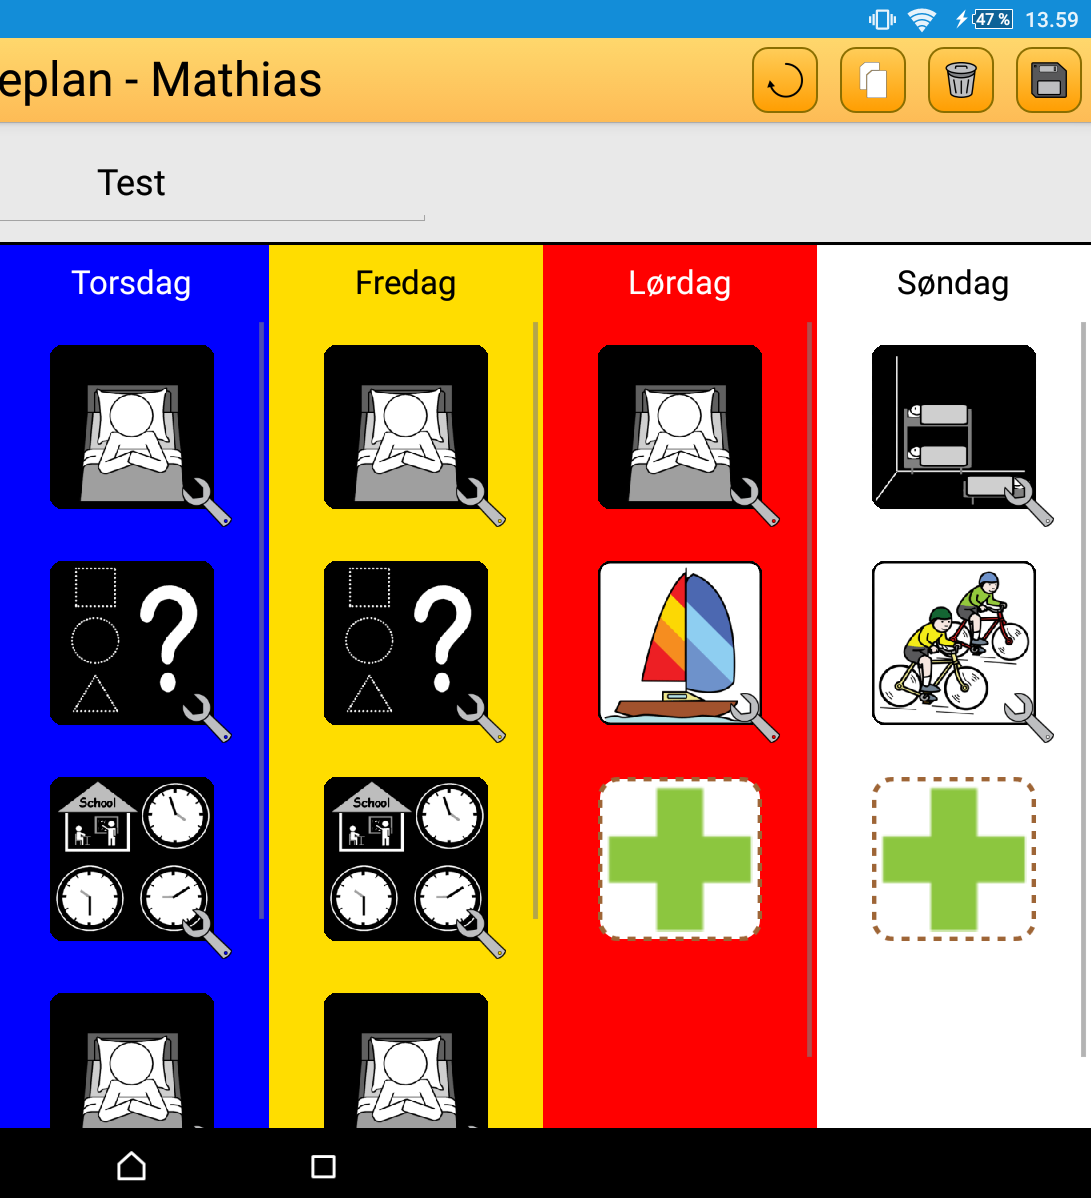
\includegraphics[width=0.5\textwidth]{figures/img/screenshots/weekplan_schedule.png}
\caption{An example of a week schedule.}
\label{fig:weekschedule}
\end{figure}

This resulted in scrolling being difficult, and needing to be changed.